\chapabstract{
This appendix highlights the post-processing approach which was required to etch metal nonidealities within silicon photonic integrated circuits. This was required due to an unexpected short within the fully integrated microwave photonic canceller. \\
\textbf{Author: Simon Bilodeau \\ Editor: Eric C. Blow} 
}
\section{Introduction}
\qquad Assume that there is a short on your metal 2 layer in your integrated layout. One can fix that by in-house post-processing. The typical metrology (e.g. reflectometer) does not work very well with a chip that has dense features like a photonic integrated circuit (PIC), but there are visual and electrical cues. 

\qquad Within Chapter 7 Silicon Microwave Photonic Cancellation, the modulators on the fully integrated design were shorted due to a design error within the M2 layer of the SiEPIC PDK (since corrected). This resulted in a resistive transfer function instead of the expected diode curve. To correct this design error, required the precise etching of a 10 $\mu m$ by 30 $\mu m$ aluminum layer microns thick without damaging the silicon photonics which laid directly below. 

\begin{figure}[!htbp]
\centering
\includegraphics[width=3in]{./Figures/AppendixB/FigB1.PNG}
\caption{Windowed lithography mask over M2 short which required etching to enable proper operation of modulator.}
\label{FigAppB1}
\end{figure}

\section{Mask Layout}
\qquad Since we want to only etch certain features, we need to define a photoresist mask over the chip. The standard Heidelberg recipe for mask making works well. Follow the Standard Operating Procedures (SOP) on the Heidelberg DWL-66+ computer. 

\textit{Note:}
\begin{enumerate}
    \item Mirror at y if you are making a mask (ignore if direct write).
    \item Strip the mask of resist before using it.
    \item In addition to desired features to etch, make sure to open the mask to other features on the chip to allow for alignment. Ideally there are features at the 4 extreme corners of the chip to align to. 
    \item Open up the mask around the wafer to easily find the chip with the mask aligner. 1 cm around the chip edge works well. 
    \item Determine where the vacuum holes on the SUSS MA6 chucks are, and make sure that the layout is offset from the center of the mask appropriately. This is only going to be an issue for very small samples. 
\end{enumerate}

\begin{figure}[!htbp]
\centering
\includegraphics[width=3.5in]{./Figures/AppendixB/mask.pdf}
\caption[Mask for PIC aluminum etching.]{Mask GDS including openings for alignment (black dashed) and openings for etching (red dashed).}
\label{FigAppB2}
\end{figure}

\section{Lithography}
\qquad The ideal thickness of resist to aim for depends on the amount of etching to be done and the selectivity of the etchant. Fortunately, we don’t have to etch much, and the acids are gentle on the resist, so we have found that the AZ1518 recipes (for ~1.9um resist thickness) to work well. A modified standard recipe with slight overetch and overdeveloping (assuming resolution is not too critical) works well.

\textit{Recipe:}
\begin{enumerate}
    \item Spin coating within photo-spincoat hoods
    \begin{enumerate}
        \item (Optional) if the sample is visibly dirty, or if you need very high resolution, clean with acetone/IPA. While aggressive cleaning of substrates is always a good idea, for precious samples like taped-out PICs better outcomes usually come out of minimizing manipulations. Note: If your PIC has edge couplers or unclad features, \textbf{DO NOT} manipulate the chip at the sensitive edge or surface. This is valid for this step and all subsequent steps.
        \item Dehydration bake of the sample, $> 1$ min at 110$^\circ$ C. Cool off on the metal plate. 
        \item Mount the sample onto a sample-sized chuck in one of the spin coaters. Center it as accurately as possible, checking with the pre-spin function. 
        \item Using a small pipette, put a few drops of AZ1518 on the sample. Cover well.
        \item Run recipe 1 (4000 RPM, 40s). Note: if the PIC has edge couplers, \textbf{DO NOT} perform the usual edge bead removal with a q-tip since this may damage the couplers.
        \item Bake at 95$^\circ$ for 1 min.
    \end{enumerate}
    \item Exposure (SUSS M6) 
    \begin{enumerate}
        \item Load sample-appropriate chuck and mask-appropriate mask holder (following machine prompt) 
        \item Exposure settings: 
        \begin{enumerate}
            \item Exposure time: 4 sec (33 \% overexposure from default) 
            \item WEC type: cont 
            \item Expose type: hard 
            \item Al gap: 50 um 
            \item HC wait: 5 secs (does not matter that much) 
        \end{enumerate}
        \item Put sample on chuck, and load into mask aligner (following machine prompt). You may read “loss of wafer vacuum” because the small sample is not covering all vacuum holes. Ignore this message. 
        \item Align the mask to the sample. Manually displace the sample on the chuck if the machine goes out of range (this is why designing for chuck vacuum hole locations is good). 
        \item Expose. Make sure the UV hits for the correct time. 
        \item Unload the sample (following machine prompt). 
    \end{enumerate}
    \item Development (Photo-develop hood) 
    \begin{enumerate}
        \item Prepare a small beaker of AZMIF300 over cleanroom wipes. You want it high and large enough to be able to gently agitate the sample during development. Note: AZMIF300 contains TMAH, handle with caution and read MSDS.
        \item Prepare a small (but larger than step a) beaker of DI water over cleanroom wipes. 
        \item Develop the sample by dipping it in the AZMIF300 beaker and gently agitating it in the solution for 1 min 15 sec (20 \% overdevelop over standard recipe). 
        \item Transfer the sample to the DI water beaker to stop development, again gently moving it for ~1 min. 
        \item Blow dry the sample with nitrogen 
        \item Hard bake at 110$^\circ$ C for 5 mins. 
        \item Inspect the exposed and developed resist with the Olympus microscope at low brightness. Note: other microscopes like the Keyence do not have UV filters and will burn your resist, even if developed. You should see windows such as in Fig. \ref{FigAppB1}.
    \end{enumerate}
\end{enumerate}
Note: Dispose of chemicals and clean up your station when you are done. 

\section{Etching}
\qquad Once the pattern is transferred onto the sample, it will stay in good condition on the order of days if not exposed to UV. If exposed to UV, it will degrade more quickly. To etch M2, we first etch the protective oxide, and then the M2 aluminum.  

Some critical notes: 
\begin{enumerate}
    \item Follow all Personal Protective Equipment (PPE) requirements, see acid hood training.
    \item BOE contains Hydrofluoric acid (HF), follow appropriate safety requirements.
    \item BOE etches glass and metal, \textbf{DO NOT} use glass beakers and metal tweezers.
    \item Aluminum Etch type A etches metal, \textbf{DO NOT} use metal tweezers.
    \item The PPE may limit mobility and visibility, practice handling tweezers and samples on dummy samples first. For instance, you do not want to accidentally scratch the resist off with your tweezers. 
\end{enumerate}

\begin{enumerate}
    \item Etch prep (Acid Hood 1) 
    \begin{enumerate}
        \item Don the appropriate PPE (see acid hood training). 
        \item Take out at least 4-5 cleanroom wipes and bring them to your station. Line 3 of them in the hood to receive 3 beakers.
        \item Install the hot plate, and set it to 50$^\circ$ C. 
        \item In a small glass beaker, poor enough Aluminum Etchant Type A so that you will be able to gently stir the sample with it remaining covered. 
        \item Put the Aluminum Etch onto the hot plate.
        \item Put DI water in a larger glass beaker. 
        \item In a small plastic beaker, pour enough BOE 10:1 so that your sample will be covered.
        \item In another plastic beaker, put DI water (more than the BOE).
        \item Wait for the Aluminum Etch to reach 50$^\circ$C, use the remote thermometer as needed. Note: Taking temperature readings is tricky, you need to reflect off the liquid: the glass beaker or the hot plate will give room temperature readings. 
        \item You should have 4 beakers, two of acid (one on the hot plate), and two of DI water.
    \end{enumerate}
    \item Oxide etch
    \begin{enumerate}
        \item Using plastic tweezers, gently deposit the sample into the BOE beaker and leave for 5 mins. Note: we have established that 5 mins is not enough to etch all the way down to M1, but will overetch M2; see thin-film interference effects on Livingstone tests Fig. \ref{FigAppB3}
        \item Rinse your tweezers at this point by dipping them in the DI water beaker and under flowing water.
        \item After 5 mins, take the sample out and gently lower it into the HF DI water for ~1 min to stop the etch. You may rinse your tweezers at this point by dipping them in the DI water beaker and under flowing water.
        \item Blow dry the sample with nitrogen 
    \end{enumerate}
    \item Metal Etch
    \begin{enumerate}
        \item Using plastic tweezers, lower the sample into the 50$^\circ$C Aluminum Etch type A solution.
        \item Keep hold of it, and gently move it around in the solution for ~8 min. Agitation and increased temperature helps with etch rate. Note: 8 mins is an overetch of M2 as evidenced by $> 10 \mu m$ lateral etching of windows, but since the solution is not significantly selective to oxide and resist, this is only a problem if you want to avoid $~10 \mu m$ wide lateral etching from your defined resist windows. 
        \item After ~8 mins, take the sample out and gently lower it into the Al Etch DI water for ~1 min to stop the etch.
        \item Blow dry the sample with nitrogen 
    \end{enumerate}
    \item Tantalum Nitride Etch
    \begin{enumerate}
        \item Thin film TaN is often used as a diffusion barrier and insulating layer between metal lines on chips \cite{Tantalum}. Tantalum nitrides are also used for thin film resistors and silicon photonics \cite{Tantalum1}. 
        \item Tantalum Etchants contain Hydrofluoric acid and will attack silicon oxides, titanium, nickel, aluminum, and chromium.
        \item Using plastic tweezers, lower sample into etchant,  
        \item Follow time on etchant. 
        \item Finish with rinse and dry.  
    \end{enumerate}
\end{enumerate}

\begin{figure}[!htbp]
\centering
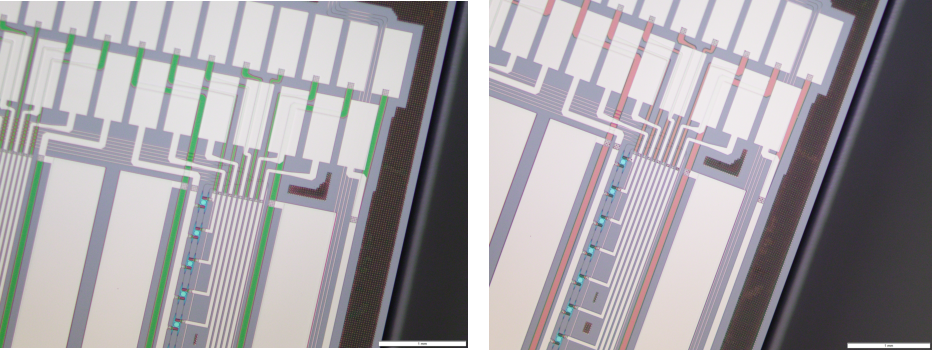
\includegraphics[width=5in]{./Figures/AppendixB/InterfermetricEtch.pdf}
\caption{Interferometric effects observed within metal layers on livingstone test.}
\label{FigAppB3}
\end{figure}

\section{Photoresist Strip}
Lastly, remove the photoresist by gently stirring the sample in acetone followed by IPA, then blow dry with nitrogen. 

\section{Results of Silicon Modulator Etch}
\qquad Fig. \ref{FigAppB4} shows the successful removal of the M2 aluminum layer shorting out the Michelson-Morley Interferometric Modulator. The low-focus imaging shows the clear removal of the metal layer while the high-focus imaging shows the lack of damage to the silicon photonics below the etched error. The success of this "chip surgery" is proven by the current-voltage (IV) measurement of the modulator. The shorted modulator showed a linear resistive curve, while the post-etched modulator showed the expected diode response, Fig. \ref{FigAppB5}. This procedure was critical for the success of the silicon microwave photonic canceller; a special thanks to Simon Bilodeau for the development and execution of this process. 

\begin{figure}[!htbp]
\centering
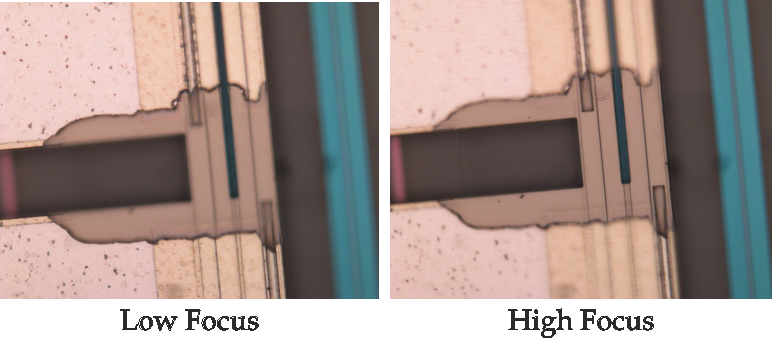
\includegraphics[width=5in]{./Figures/AppendixB/TiEtch.pdf}
\caption[Imaging of successful etch in varying imaging focus to highlight different chip depths.]{Etched M2 short in low (left) and high (right) focus highlighting the removal of the aluminum layer as well as the unaltered optical components below.}
\label{FigAppB4}
\end{figure}

\begin{figure}[!htbp]
\centering
\includegraphics[width=5.5in]{./Figures/AppendixB/IVetch.pdf}
\caption[Experimental data confirming successful etch.]{Measured resistive IV curve of modulator before etch (left) and measured diode curve of modulator after successful aluminum etch (right).}
\label{FigAppB5}
\end{figure}

\qquad \textit{Note:} Before etching, the authors attempted to electrically open the modulator by passing a short pulse of high (2 Amp) current. This idea was neither effective nor well-thoughout; it did not work. The probes melted to the electrical pads before the electrical proprieties of the device changed. 
